%%%%%%%%%%%%%%%%%%%%%%%%%%%%%%%%%%%%%%%%%
% University/School Laboratory Report
% LaTeX Template
% Version 3.1 (25/3/14)
%
% This template has been downloaded from:
% http://www.LaTeXTemplates.com
%
% Original author:
% Linux and Unix Users Group at Virginia Tech Wiki 
% (https://vtluug.org/wiki/Example_LaTeX_chem_lab_report)
%
% License:
% CC BY-NC-SA 3.0 (http://creativecommons.org/licenses/by-nc-sa/3.0/)
%
%%%%%%%%%%%%%%%%%%%%%%%%%%%%%%%%%%%%%%%%%

%----------------------------------------------------------------------------------------
%	PACKAGES AND DOCUMENT CONFIGURATIONS
%----------------------------------------------------------------------------------------

\documentclass{article}

\usepackage[version=3]{mhchem} % Package for chemical equation typesetting
\usepackage{siunitx} % Provides the \SI{}{} and \si{} command for typesetting SI units
\usepackage{graphicx} % Required for the inclusion of images
\usepackage{natbib} % Required to change bibliography style to APA
\usepackage{amsmath} % Required for some math elements 
\usepackage{enumerate} % Required for the enumerate function
\usepackage[siunitx]{circuitikz} % Required for the drawing of circuit diagrams
\usepackage{caption}
\usepackage{graphicx}
\usepackage{subcaption}
\usepackage{xfrac}
\usepackage{float}
\usepackage{enumitem}
\usepackage{chemgreek}
\usepackage{pgfplots}
\usepackage{booktabs}
\usepackage[]{mcode}
\usepackage{epstopdf}

\setlength\parindent{0pt} % Removes all indentation from paragraphs

\renewcommand{\labelenumi}{\alph{enumi}.} % Make numbering in the enumerate environment by letter rather than number (e.g. section 6)

%\usepackage{times} % Uncomment to use the Times New Roman font

%----------------------------------------------------------------------------------------
%	DOCUMENT INFORMATION
%----------------------------------------------------------------------------------------

\title{Communication Systems \\ Experiment 1 \\ ENG473} % Title

\author{Shane \textsc{Reynolds}} % Author name

\date{\today} % Date for the report

\begin{document}

\maketitle % Insert the title, author and date

\begin{center}
\begin{tabular}{l r}
Date Performed: & July 29, 2016 \\ % Date the experiment was performed
Instructor: & Dr Sina Vafi % Instructor/supervisor
\end{tabular}
\end{center}

% If you wish to include an abstract, uncomment the lines below
% \begin{abstract}
% Abstract text
% \end{abstract}

\graphicspath{{./fig/}}

%----------------------------------------------------------------------------------------
%	SECTION 1
%----------------------------------------------------------------------------------------

\section{Objective}

Investigate the Universal Datagram Protocol (UDP) gaining an understanding of the basic functionality and the protocol performance using a peak signal to noise ratio metric.

%----------------------------------------------------------------------------------------
%	SECTION 2
%----------------------------------------------------------------------------------------

\section{Part 1: Process \& Results}

A basic network was simulated using Matlab. A script which created an actor playing the role of server was created. A second script was created to create an actor which played to role of the client in the network simulation. Both scripts can be seen in Appendix A. 

The server side of the simulation sends a string using UDP to the 25000 port on the local host, and the client side listens at port 25000 on the local host data. Using two instances of Matlab the client side script was executed first, followed by the server script in the second instance of Matlab. The following output was recorded in the Matlab instance running the client script:\\
\begin{verbatim}
	This is the first project of ENG 473 relevant to UDP 
	transmission of some characters...
\end{verbatim}

\newpage
%----------------------------------------------------------------------------------------
%	SECTION 3
%----------------------------------------------------------------------------------------

\section{Part 2: Process, Results \& Discussion}

A basic network was again simulated using Matlab, however, this time an image was sent using UDP. The simulation was designed similarly to the simulation in part 1: a client-side actor and a server-side actor was established in the simulation. An image was loaded into the simulation. the image was discretised into 786432 blocks, which were stored in a vector.

\begin{table}[h]
	\caption{results from simulation using different SNR values}
	\hspace{0.85cm}
	\begin{minipage}{0.48\textwidth}
		\begin{tabular}{c c}
			\toprule
			SNR(dB) & PSNR(dB)\\
			\midrule
			0.10	& 47.9041	\\
			0.50	& 48.2652	\\
			1.00	& 48.7386	\\
			1.00	& 27.0312	\\
			1.25	& 48.9427	\\
			1.25	& 48.9461	\\
			1.50	& 49.1585	\\
			1.50	& 29.4448	\\
			1.50	& 25.7043	\\
			2.00	& 25.7342	\\
			2.00	& 29.6410	\\
			2.00	& 49.6027	\\
			2.50	& 49.5950	\\
			2.50	& 26.2564	\\
			2.50	& 25.6747	\\
			2.50	& 27.3277	\\
			3.00	& 50.4571	\\
			3.00	& 50.4518	\\
		\end{tabular}
	\end{minipage}
	\begin{minipage}{0.48\textwidth}
		\begin{tabular}{c c}
			\toprule
			SNR(dB) & PSNR(dB)\\
			\midrule
			3.00	& 50.4564	\\
			3.00	& 50.4432	\\
			3.25	& 50.6651	\\
			3.25	& 50.6523	\\
			3.25	& 50.6738	\\
			3.25	& 50.6634	\\
			3.50	& 50.8649	\\
			3.50	& 50.8788	\\
			3.50	& 50.8686	\\
			3.50	& 50.8694	\\
			3.75	& 51.0798	\\
			3.75	& 26.7202	\\
			3.75	& 26.2578	\\
			3.75	& 29.3694	\\
			4.00	& 29.6583	\\
			4.00	& 34.1350	\\
			4.00	& 51.2722	\\
			4.00	& 51.2898	\\
		\end{tabular}
	\end{minipage}
\end{table}

Noise was artificially introduced to each stored block of the image using a Gaussian white noise process. The severity of the random noise was measured by the signal to noise ratio (SNR). The server side actor then took each block in the vector and sent it to port 25000 on the local host using UDP. The information was received by the client-side actor, and the image reconstructed. Finally, a comparison was made between the reconstructed and original images using the peak signal to noise ratio (pnsr). The simulation was repeated for a number of different SNR values, the results of which can be seen in Table 1.\\

The quality of the reconstructed image improved as the SNR increased, however, the actual reconstructed image bore no visually discernible difference to the original image. This was true for all of the reconstructed images, irrespective of the SNR. Figure 1 shows  the original image on the left and a reconstructed image with a PSNR of 26.72dB on the right.
  
\begin{figure}[H]
	\centering
	\begin{minipage}{0.48\textwidth}
		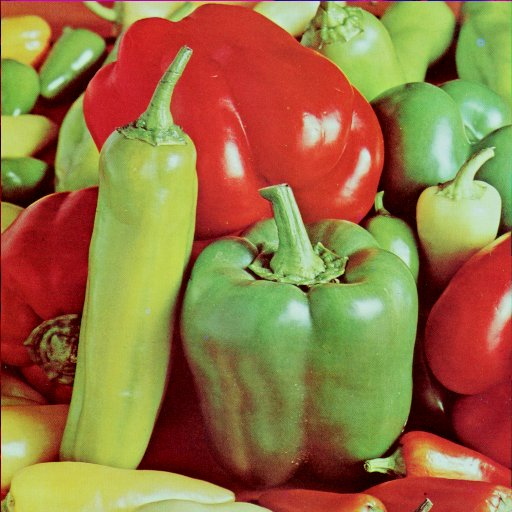
\includegraphics[scale=0.3]{Peppers.jpg}
	\end{minipage}
	\begin{minipage}{0.48\textwidth}
		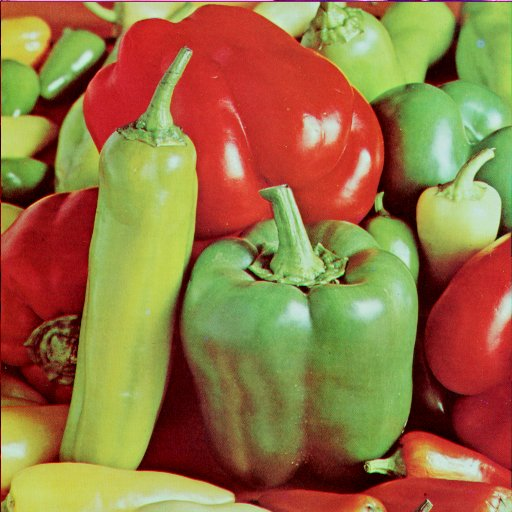
\includegraphics[scale=0.3]{Peppers_new_SNR_3.jpg}
	\end{minipage}
	\caption{The original image is on the left and the transmitted image is on the right. The transmitted image has a PSNR of 26.72 dB.}
\end{figure}

 Average PSNR values were calculated for the SNR values which were simulated multiple times. The results were plotted in Figure 2. There is no clear pattern that can be distinguished from the observed results in the graph. The PSNR is an image quality metric - the higher the PNSR, the more a reconstructed image resembles the original image. It could be hypothesised that as the SNR increases we would expect to see an increase in the PSNR, however, in this instance there may simply be too few samples for each individual SNR which has resulted in the stochasticity of the simulation overwhelming the results.
 
 \begin{figure}[h]
 	\centering
 	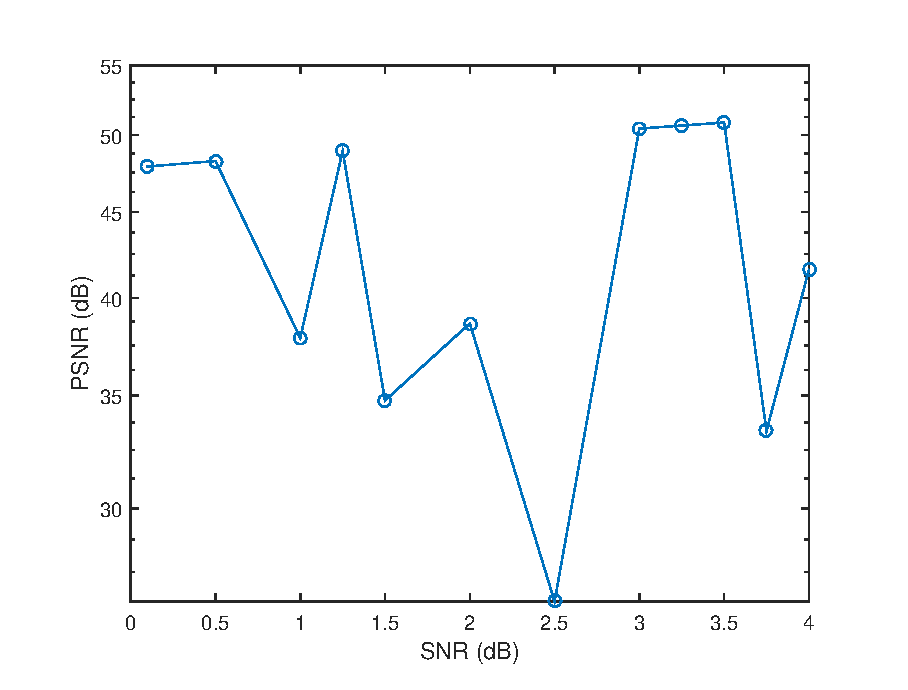
\includegraphics[scale=0.65]{fig1.eps}
 	\caption{Plot of simulation results}
 \end{figure}

Despite the fact the images have no visible degradation, there has been some loss of quality from the transmission and reconstruction. One way that we might improve this is to use a different protocol on the transmission layer of our network. A competing protocol, which is used extensively in networking, is Transmission Control Protocol (TCP). TCP differs from UDP in that UDP is what's known as connectionless, whilst TCP is not. This means that the UDP server will send the information whether the client is ready or not. In contrast, TCP will establish a connection with the client prior to sending information. It is this connection that allows TCP to ensure that no packets are lost or corrupted - if the server does not receive a suitable acknowledgement from the receiver, then the packet is resent by the server and the corrupt packet dropped at the receiver. This may make TCP a better candidate for the purpose of the transmission of this image, or any other purpose where speed is not a core requirement of the transmission.


%----------------------------------------------------------------------------------------
%	SECTION 5
%----------------------------------------------------------------------------------------

\section{Conclusion}

A network simulation was performed using a single server and client pair. The server used UDP to send packets of information of an image to the client with Gaussian white noise introduced. It was hypothesised that the higher the SNR, the higher the PNSR and the better quality the image reconstruction. Data collected from the simulation was inconclusive in determining whether this was the case. TCP was highlighted as an alternative to UDP, which would be more reliable in delivering quality images due to the fact that TCP requires a connection between the server and the client prior to data transmission. 

\newpage

%----------------------------------------------------------------------------------------
%	APPENDIX A
%----------------------------------------------------------------------------------------

\section{Appendix A}

An actor playing the role of server was created with the following script:

\begin{lstlisting}
% This code is for the server side of our UDP transsion
% Clear the workspace and any variables
clear; clc; close all;
hudps = dsp.UDPSender('LocalIPPortSource','Auto', 'RemoteIPAddress',...
'127.0.0.1','RemoteIPPort',25000);
%hudps = dsp.UDPSender;


% Store the transmission string in an appropriate variable
transmission_string = ['This is the first project of ENG 473 ' ...
'relevant to UDP transmission ' ...
'of some characters...!'];

% Convert the string to uint8
data = uint8(transmission_string);
for i=1:size(data,2)
	step(hudps,data(i))%send the elements 1 by 1
end

release(hudps)
\end{lstlisting}

An actor was created which played to role of the client in the network simulation. The Matlab implementation is shown below:

\begin{lstlisting}
% Clear the workspace and any stored variables
clear; clc; close all;
hudpr = dsp.UDPReceiver('RemoteIPAddress','0.0.0.0','LocalIPPort',...
25000,'MessageDataType','uint8');
%hudpr = dsp.UDPReceiver;

string=[];
count=1;
eof=0;

while(~eof)
	%disp('in loop')
	dataReceived = step(hudpr);
	if strcmp(char(dataReceived),'!')
		eof=1; % ! signified the end
	else
		string = [string char(dataReceived)]; %fill the string
		count=count+1;
	end
end

disp(string) %display the string
release(hudpr)
\end{lstlisting}

\newpage

%----------------------------------------------------------------------------------------
%	APPENDIX B
%----------------------------------------------------------------------------------------

\section{Appendix B}

The following script was used to automate the lengthy process and record the results and transmitted images:

\begin{lstlisting}
% Clear the workspace and any variables
clc; clear;

% Create file name
file_stem = ['C:\Users\Shane Reynolds\Google Drive\'...
'University\Charles Darwin University\'...
'Communication Systems\Assignment 1\'];
file = 'Peppers.tiff';
file_name = strcat(file_stem,file);

% Read an image from the graphical file.
[data,map] = imread(file_name);
str3 = sprintf('Read an image from the graphical file...');
disp(str3);

% Return the size of read image file.
[a,b,c]=size(data);

% The overall number of 'data'
sz_data=a*b*c;
str4 = sprintf('Size of file is: %2.2d', sz_data);
disp(str4);

% The 'data' obtained from ‘imread’ is a three dimensional matrix.
% Use reshape to convert it into a two dimensional matrix based on
% only one row. we call this reshaped matrix as 'T' matrix
T = reshape(data,1,a*b*c); 

SNR_vec = [0.1 0.5 1.0 1.0 1.25 1.25 1.5 1.5 1.5 2.0 2.0 2.0 2.0 ...
2.5 2.5 2.5 3.0 3.0 3.0 3.0 3.25 3.25 3.25 3.25 ...
3.5 3.5 3.5 3.5 3.75 3.75 3.75 3.75 4.0 4.0 4.0 4.0];

inst_vect = [1 1 1 2 1 2 1 2 3 1 2 3 1 2 3 4 1 2 3 4 ...
1 2 3 4 1 2 3 4 1 2 3 4 1 2 3 4 ];
qty_img = [];

for j=1:length(SNR_vec)

	% Initialise udp sender and reciever
	hudps = dsp.UDPSender('RemoteIPPort',25000); 
	hudpr = dsp.UDPReceiver('LocalIPPort',25000);
	str1 = sprintf('Succesfully initialise udp sender and reciever...');
	disp(str1);

	% Set a value as signal to noise ratio (in dB)
	SNR = SNR_vec(j);
	inst = inst_vect(j);
	str2 = sprintf('Set signal to noise ratio to: %2.2d', SNR);
	disp(str2);


	% Make a loop for transmitting 'data' with size of
	% sz_data, one by one
	fprintf('Processing')
	for i=1:sz_data
		% this 'if' command types value of i and helps you to
		% understand execution steps of your program
		if rem(i-1,100000)==0
			fprintf('.')
		end

		% awgn adds noise to 'T'.
		T_dmg(i)=awgn(T(i),SNR);

		% 'Noisy formed 'T' (T_dmg) is converted to 8-bit unsigned integer
		dataSent = uint8(T_dmg(i));

		% Obtained '8-bit unsigned integer (dataSent)' is transmitted by
		% udp protocol.
		step(hudps, dataSent);

		% transmitted data is received by udp protocol
		dataReceived = step(hudpr)';

		% This and following three lines help us to save valid received
		% data in an array. We check validity of the data by isempty command.
		flg = isempty(dataReceived);
		if flg~=1 
			% Received data is saved in an array. This is the received image.
			d_rec(i) = dataReceived;
		end
	end

	fprintf('\n')
	% terminate udp transmitter and the udp receiver
	release(hudps);
	release(hudpr);

	% reshape received data to three dimensional array matched with the
	% structure of the image read.
	A = reshape(d_rec,a,b,c); 

	% write the received image to a graphical file. The name of this file is
	% ‘Peppers_new_SNR_0.1_1.tiff. Again, type the correct path for saving this
	% image file on you your computer.
	new_file = strcat('Peppers_new_SNR_',num2str(SNR),'_', ...
	num2str(inst),'.tiff');
	new_file_name = strcat(file_stem,new_file);
	imwrite(A,new_file_name);

	% Compares quality of the received image with original one
	qty_img(j) = psnr(A,data);
	str6 = sprintf('Quality of recieve image compared to original: %2.2d', ...
	qty_img(j));
	disp(str6);
	disp('***************************************************************')
end
\end{lstlisting}

\end{document}